\documentclass[12pt,a4paper]{article}
\usepackage[margin=1in]{geometry}
\usepackage{graphicx,booktabs,longtable,array,xcolor,hyperref,float,caption,enumitem,listings,pgfgantt}
\usepackage[T1]{fontenc}\usepackage{amsmath}\usepackage{tikz}
\usetikzlibrary{arrows.meta,positioning,shapes.geometric,shapes.multipart,fit,calc}
\hypersetup{colorlinks=true,linkcolor=blue,urlcolor=blue}
\setlength{\parskip}{4pt}
\lstset{basicstyle=\ttfamily\footnotesize,breaklines=true,frame=single,numbers=left,numberstyle=\tiny,keywordstyle=\color{blue}}

% ---- Fill this from FFWC station data (e.g. Bahadurabad / Porabari) ----

\begin{document}

%================ TITLE PAGE ================
\begin{titlepage}
\centering
{\large Mawlana Bhashani Science and Technology University\\
Department of Information and Communication Technology\\[1.5cm]}
{\Large\bfseries Software Engineering and Project Management\\[0.3cm]}
{\large Project Proposal\\[1.5cm]}
\rule{\textwidth}{1.5pt}\\[0.4cm]
{\LARGE\bfseries FloodGuard: IoT-Based Flood Early Warning System for Riverside Villages\\[0.4cm]}
\rule{\textwidth}{1.5pt}\\[1.5cm]
\begin{tabular}{rl}
\textbf{Submitted by:} & Jubayer Ahmed\\
\textbf{ID:} & IT24027\\
\textbf{Session:} & 2023--2024\\
\textbf{Level:} & 3rd Year, 1st Semester\\[0.6cm]
\textbf{Submitted to:} & Professor Dr.\ Md.\ Ziaur Rahman\\
 & Department of ICT, MBSTU\\[0.6cm]
\textbf{Date:} & \today
\end{tabular}
\end{titlepage}

\tableofcontents
\newpage

%================ ABSTRACT ================
\section*{Abstract}
\addcontentsline{toc}{section}{Abstract}
Bangladesh faces recurrent floods, and riverside communities along the Jamuna, including areas of Tangail, often receive warnings late or in a form that does not reach households. This proposal presents \textbf{FloodGuard}, a low-cost Internet of Things (IoT) system that measures river water level with an ESP32 microcontroller and an ultrasonic sensor, transmits the readings over WiFi (HTTP) to a Java Servlet server, classifies the situation as \emph{Safe}, \emph{Warning} or \emph{Danger} against a configurable danger level, and notifies people through a web dashboard, local LED/buzzer indicators and Telegram messages. The project follows the Incremental process model over 12 weeks. The proposal contains the problem analysis, requirements, SWOT, feasibility, risk and cost analysis, schedule with Gantt chart, six UML diagrams, and a simple web interface implemented with more than five classes from the class diagram.

\medskip\noindent\textbf{Keywords:} IoT, ESP32, flood early warning, Java Servlet, ultrasonic sensor, Incremental model, UML.

%================ 1 INTRODUCTION ================
\section{Introduction}
Floods are among the most frequent natural disasters in Bangladesh. The Brahmaputra--Jamuna river system regularly rises above its danger level during the monsoon, affecting districts such as Kurigram, Gaibandha, Jamalpur, Sirajganj and Tangail. The Flood Forecasting and Warning Centre (FFWC) of the Bangladesh Water Development Board (BWDB) publishes daily bulletins for monitored stations, but these are station-level and national-scale products. Village-level, automatic and immediate alerts remain limited.

Advances in low-cost microcontrollers (e.g.\ ESP32), cheap sensors and free software make it feasible to build a local monitoring and alerting node. FloodGuard is a prototype of such a node and the software that receives, analyses and communicates its data.

\section{Problem Statement}
\begin{itemize}[noitemsep]
\item Water level monitoring at village scale is mostly manual and irregular.
\item Official bulletins are periodic and do not directly reach every household.
\item Residents and volunteers have no automatic, threshold-based alert tied to their nearest river point.
\item Existing solutions are costly or require specialised infrastructure, which is difficult for a student or small community project.
\end{itemize}
\textbf{Proposed solution:} an IoT-based, low-cost system that continuously measures water level, evaluates it against the danger level, records history and issues staged alerts (Safe/Warning/Danger).

\section{Objectives}
\subsection{General objective}
To design and develop a low-cost IoT-based early warning prototype that monitors river water level and issues timely flood alerts.
\subsection{Specific objectives}
\begin{enumerate}[noitemsep]
\item To measure water level using an ESP32 and an ultrasonic sensor (HC-SR04 / JSN-SR04T).
\item To transmit readings to a Java Servlet server over WiFi using HTTP.
\item To classify status as Safe ($<$80\%), Warning (80--100\%) and Danger ($\ge$100\%) of the danger level.
\item To display live status, graph and alert history on a web dashboard.
\item To generate local alarms (LED, buzzer) and notifications (console SMS simulation, Telegram).
\item To apply software engineering practice: Incremental model, UML modelling, testing and documentation.
\end{enumerate}

\section{Scope and Limitations}
\subsection{In scope}
Single-river-point monitoring node; server-side processing; web dashboard; alert generation and history; user roles (Admin, Volunteer, Resident); simulated and real sensor input; UML design; LaTeX documentation.
\subsection{Out of scope}
Hydrological forecasting/machine learning; nationwide deployment; real SMS-gateway billing integration; mobile application; weatherproof field enclosure and solar power design (discussed as future work).
\subsection{Limitations}
The prototype is demonstrated by emulating water level (sensor distance variation in Wokwi or on a bench) and does not claim live river measurement. FloodGuard is a decision-support aid and does not replace official FFWC forecasts.

%================ 2 LITERATURE ================
\section{Literature Review and Existing Systems}
\begin{itemize}[noitemsep]
\item \textbf{FFWC / BWDB:} operates the national flood forecasting service and publishes daily water level bulletins and danger levels for monitored river stations. It is authoritative but not a village-level automatic alerting service.
\item \textbf{Mobile/SMS flood alerts:} government and NGO-supported services broadcast warnings, usually based on official forecasts rather than a local sensor.
\item \textbf{IoT water level monitoring:} many academic and hobby systems combine ESP8266/ESP32 with ultrasonic sensors and cloud dashboards. Typical gaps are limited alert staging, no role-based users and no structured software engineering documentation.
\item \textbf{Messaging APIs:} the Telegram Bot API provides free programmatic notifications.
\end{itemize}
\textbf{Gap addressed:} a low-cost, locally deployable node that links sensing, server-side rules, history, role-based users and multi-channel alerts, designed and documented with a formal process.

%================ 3 SWOT ================
\section{SWOT Analysis}
\begin{table}[H]\centering\small
\begin{tabular}{p{0.47\textwidth}p{0.47\textwidth}}
\toprule
\textbf{Strengths} & \textbf{Weaknesses}\\\midrule
Real and important local problem; low cost; real-time alerts; simple technology (Java, ESP32); scalable to more nodes; strong SE structure &
Prototype uses emulated water level; depends on WiFi and power; no forecasting; single-person effort; sensor accuracy not validated in field\\\midrule
\textbf{Opportunities} & \textbf{Threats}\\\midrule
Interest from BWDB/NGOs/disaster management; rising climate-related flood risk; high mobile penetration; cheap IoT hardware (ESP32, LoRa); open weather APIs; future research &
False or missed alerts; sensor damage/theft in floods; network and power outage; overlap with existing official system; maintenance funding\\\bottomrule
\end{tabular}
\caption{SWOT analysis of FloodGuard}
\end{table}
\noindent\textbf{Mitigation:} use GSM/LoRa and local siren where internet is unavailable; battery/solar backup; averaging and outlier filtering of readings; position FloodGuard as a village-level complement to FFWC.

%================ 4 REQUIREMENTS ================
\section{Requirements Specification}
\subsection{Functional requirements}
\begin{longtable}{@{}lp{0.85\textwidth}@{}}
\toprule\textbf{ID} & \textbf{Requirement}\\\midrule\endhead
FR1 & The system shall receive water level readings from the ESP32 node via HTTP POST.\\
FR2 & The system shall store each reading with a timestamp.\\
FR3 & The system shall compute status (Safe/Warning/Danger) using the river's danger level.\\
FR4 & The system shall generate an alert when the status changes to Warning or Danger.\\
FR5 & The system shall display current level, status colour, progress bar and history graph on a dashboard.\\
FR6 & The system shall show the alert list with time, village, level and message.\\
FR7 & The Admin shall manage rivers, sensors, villages and users.\\
FR8 & Residents and Volunteers shall be able to register and receive notifications.\\
FR9 & The system shall support role-based login (Admin, Volunteer, Resident).\\
FR10 & The ESP32 shall show status with green/yellow/red LEDs and a buzzer.\\
FR11 & The system shall send Telegram and simulated SMS notifications, only on status change.\\\bottomrule
\end{longtable}
\subsection{Non-functional requirements}
\begin{longtable}{@{}lp{0.85\textwidth}@{}}
\toprule\textbf{ID} & \textbf{Requirement}\\\midrule\endhead
NFR1 & \textbf{Performance:} status update visible within 5 seconds of a reading.\\
NFR2 & \textbf{Reliability:} local LED/buzzer alert works without internet; server must not crash if Telegram fails.\\
NFR3 & \textbf{Usability:} simple dashboard usable on a mobile browser.\\
NFR4 & \textbf{Security:} credentials and tokens not stored in source code; device key to validate readings; passwords hashed.\\
NFR5 & \textbf{Maintainability:} layered design (Servlet--Service--DAO); danger level configurable.\\
NFR6 & \textbf{Portability:} runs on any Servlet container (Jetty/Tomcat) and JDK 17+.\\
NFR7 & \textbf{Cost:} prototype hardware under approximately BDT 1{,}100.\\\bottomrule
\end{longtable}
\subsection{Input and output}
\textbf{Inputs:} water level (sensor), river/village/user details (Admin, Residents), login credentials, simulation start. \textbf{Outputs:} dashboard (status, graph), alert list, LED/buzzer, Telegram and simulated SMS, stored history.

%================ 5 FEASIBILITY ================
\section{Feasibility Study}
\begin{itemize}[noitemsep]
\item \textbf{Technical:} ESP32, HC-SR04, Java, Maven, Jetty, Chart.js are mature and well documented; the developer has prior Servlet experience. Feasible.
\item \textbf{Economic:} software is free; hardware is about BDT 750--1{,}100 or BDT 0 using Wokwi simulation. Feasible.
\item \textbf{Operational:} simple colour-coded dashboard and messages are easy for volunteers and villagers.
\item \textbf{Schedule:} 12 weeks with three increments is realistic.
\item \textbf{Legal/ethical:} no sensitive personal data beyond name/phone; stored with restricted access.
\end{itemize}

%================ 6 RISK ================
\section{Risk Analysis}
\begin{table}[H]\centering\small
\begin{tabular}{@{}p{0.3cm}p{4.3cm}p{1.8cm}p{1.6cm}p{5.6cm}@{}}
\toprule \# & \textbf{Risk} & \textbf{Probability} & \textbf{Impact} & \textbf{Mitigation}\\\midrule
1 & Sensor noise / wrong reading & Medium & Medium & Average several samples; reject outliers\\
2 & No internet at demo/site & High & High & Phone hotspot; LED/buzzer local alert; console fallback\\
3 & Telegram token leak & Medium & High & Environment variables; \texttt{.gitignore}; revoke token\\
4 & Hardware delay/failure & Medium & Medium & Wokwi simulation and Java simulator as backup\\
5 & Fake data posted to server & Low & Medium & Device API key; range validation\\
6 & Alert spam & Medium & Low & Notify only on status change\\
7 & Schedule overrun & Medium & Medium & Incremental delivery; keep scope simple\\
8 & Power outage in field & High & High & Battery/solar (future work)\\
9 & Misuse as official forecast & Low & High & Clear disclaimer in UI and report\\\bottomrule
\end{tabular}
\caption{Risk register}
\end{table}

%================ 7 COST ================
\section{Cost and Resource Estimation}
\begin{table}[H]\centering\small
\begin{tabular}{@{}lcr@{}}
\toprule \textbf{Item} & \textbf{Qty} & \textbf{Approx.\ cost (BDT)}\\\midrule
ESP32 development board & 1 & 450--650\\
HC-SR04 ultrasonic sensor & 1 & 100--150\\
LEDs (G/Y/R) + 220$\Omega$ resistors & 3+3 & 20--30\\
Active buzzer & 1 & 20--40\\
Breadboard + jumper wires & 1 set & 150--250\\
\midrule \textbf{Hardware total (optional)} & & \textbf{about 750--1{,}100}\\
Software (IntelliJ Community, Maven, Jetty, MySQL, Git, Overleaf, Wokwi, Telegram Bot) & & 0\\\bottomrule
\end{tabular}
\caption{Estimated prototype cost (prices vary; verify locally)}
\end{table}
\noindent\textbf{Human resource:} one developer, about 8--10 hours per week for 12 weeks. A field deployment would additionally need weatherproof enclosure, solar panel, battery and GSM/LoRa module, estimated separately per node.

%================ 8 PROCESS MODEL ================
\section{Software Process Model: Incremental Model}
\subsection{Reason for selection}
Requirements are reasonably clear, but the system has separable parts (data pipeline, dashboard, alerting). The Incremental model delivers a working product early and adds functionality in each increment, which reduces risk for a single-developer, time-boxed project.

\subsection{Increments}
\begin{table}[H]\centering\small
\begin{tabular}{@{}p{2.2cm}p{7cm}p{5cm}@{}}
\toprule \textbf{Increment} & \textbf{Content} & \textbf{Output}\\\midrule
Planning \& Design & Problem analysis, requirements, schedule, UML & Proposal, diagrams\\
Increment 1 & Servlet \texttt{/data}, River/Sensor/Reading/Alert classes, status logic, storage & Working data pipeline\\
Increment 2 & Dashboard (colours, progress bar, Chart.js graph), alert list, simulation button & Live dashboard\\
Increment 3 & Role-based login, notifications (console/Telegram), ESP32 + LEDs/buzzer, Wokwi & Complete prototype\\
Testing \& Closure & JUnit and system tests, report, GitHub release & Final submission\\\bottomrule
\end{tabular}
\caption{Increments}
\end{table}

\subsection{Weekly schedule}
\begin{table}[H]\centering\small
\begin{tabular}{@{}lp{9.5cm}l@{}}
\toprule \textbf{Week} & \textbf{Activity} & \textbf{Milestone}\\\midrule
1--2 & Idea finalisation, problem analysis, requirements, SWOT & M1\\
2--3 & Process model, schedule, Gantt chart & M2\\
3--5 & UML diagrams (DFD, Use case, Activity, ER, Class, Object) & M3\\
5--7 & Increment 1: Servlet, model classes, storage & M4\\
7--9 & Increment 2: dashboard, chart, alerts list & M5\\
9--10 & Increment 3: login, Telegram, ESP32/Wokwi & M6\\
10--11 & Testing and bug fixing & M7\\
11--12 & Final report (LaTeX), GitHub, submission & M8\\\bottomrule
\end{tabular}
\caption{Project schedule}
\end{table}

\subsection{Milestones and deliverables}
\begin{table}[H]\centering\small
\begin{tabular}{@{}llp{7.5cm}l@{}}
\toprule \textbf{ID} & \textbf{Milestone} & \textbf{Deliverable} & \textbf{Week}\\\midrule
M1 & Requirements complete & Requirements document, SWOT & 2\\
M2 & Plan approved & Schedule, Gantt chart, risk register & 3\\
M3 & Design complete & Six UML diagrams & 5\\
M4 & Increment 1 done & Data pipeline, source code & 7\\
M5 & Increment 2 done & Dashboard with graph and alerts & 9\\
M6 & Increment 3 done & Integrated system, ESP32 code, Wokwi project & 10\\
M7 & Testing done & Test cases and report & 11\\
M8 & Final submission & Proposal/report PDF, GitHub repository & 12\\\bottomrule
\end{tabular}
\caption{Milestones and deliverables}
\end{table}

\subsection{Gantt chart}
\begin{figure}[H]\centering
\resizebox{\textwidth}{!}{%
\begin{ganttchart}[hgrid,vgrid,x unit=0.55cm,y unit chart=0.6cm,title height=1,bar/.append style={fill=blue!50},milestone/.append style={fill=red}]{1}{12}
\gantttitle{Weeks}{12}\\
\gantttitlelist{1,...,12}{1}\\
\ganttbar{Requirements \& SWOT}{1}{2}\\
\ganttbar{Process model \& Gantt}{2}{3}\\
\ganttbar{UML diagrams}{3}{5}\\
\ganttbar{Increment 1}{5}{7}\\
\ganttbar{Increment 2}{7}{9}\\
\ganttbar{Increment 3}{9}{10}\\
\ganttbar{Testing}{10}{11}\\
\ganttbar{Report \& GitHub}{11}{12}\\
\ganttmilestone{M1}{2}\ganttmilestone{M2}{3}\ganttmilestone{M3}{5}\ganttmilestone{M4}{7}\ganttmilestone{M5}{9}\ganttmilestone{M6}{10}\ganttmilestone{M7}{11}\ganttmilestone{M8}{12}
\end{ganttchart}}
\caption{Gantt chart (12 weeks)}
\end{figure}

%================ 9 ARCHITECTURE ================
\section{System Architecture and Technology Stack}
\begin{figure}[H]\centering
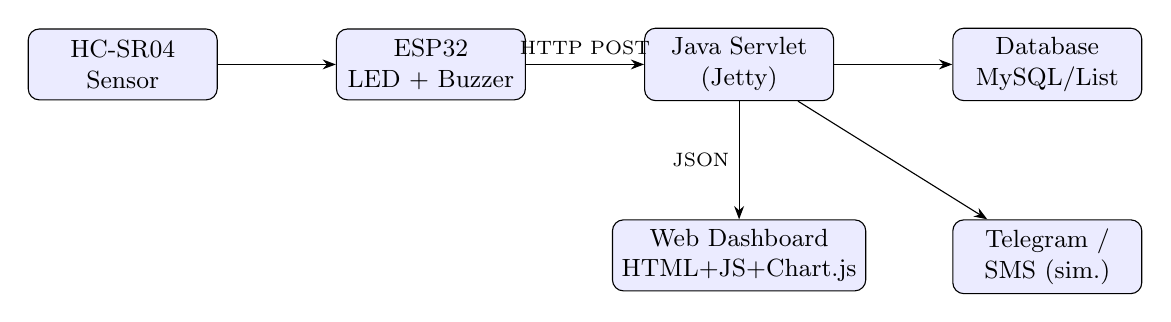
\begin{tikzpicture}[node distance=1.5cm,box/.style={draw,rounded corners,align=center,minimum width=2.4cm,minimum height=0.9cm,fill=blue!8,font=\small},>=Stealth]
\node[box](s){HC-SR04\\Sensor};
\node[box,right=of s](e){ESP32\\LED + Buzzer};
\node[box,right=of e](v){Java Servlet\\(Jetty)};
\node[box,right=of v](d){Database\\MySQL/List};
\node[box,below=of v](w){Web Dashboard\\HTML+JS+Chart.js};
\node[box,below=of d](t){Telegram /\\SMS (sim.)};
\draw[->](s)--(e);\draw[->](e)--node[above,font=\scriptsize]{HTTP POST}(v);
\draw[->](v)--(d);\draw[->](v)--node[left,font=\scriptsize]{JSON}(w);\draw[->](v)--(t);
\end{tikzpicture}
\caption{FloodGuard architecture}
\end{figure}
\begin{table}[H]\centering\small
\begin{tabular}{@{}ll@{}}\toprule \textbf{Layer} & \textbf{Technology}\\\midrule
Device & ESP32, HC-SR04/JSN-SR04T, LEDs, buzzer (Arduino C++); Wokwi simulator\\
Backend & Java 17, Jakarta Servlet, DAO pattern, Maven, Jetty\\
Database & ArrayList (initial), MySQL/SQLite\\
Frontend & HTML, CSS, JavaScript, Chart.js\\
Notification & Console SMS simulation, Telegram Bot API\\
Tools & IntelliJ IDEA, Git/GitHub, Overleaf, PlantUML/TikZ, JUnit\\\bottomrule
\end{tabular}\end{table}
\noindent\textbf{Water level formula:} with sensor height $H$ above the river bed and measured distance $d$, $\text{level}=H-d$. \textbf{Status rule:} $p=\text{level}/\text{DangerLevel}\times100$; Safe if $p<80$, Warning if $80\le p<100$, Danger if $p\ge100$. The danger level is taken from FFWC station data and is configurable.

%================ 10 UML ================
\section{UML Diagrams}

\subsection{Data Flow Diagram (Level 0 and Level 1)}
\begin{figure}[H]\centering
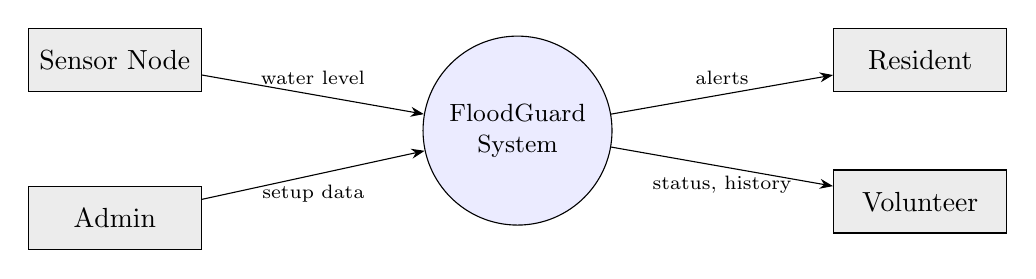
\begin{tikzpicture}[ent/.style={draw,minimum width=2.2cm,minimum height=0.8cm,fill=gray!15},proc/.style={draw,circle,align=center,minimum size=2.4cm,fill=blue!8,font=\small},>=Stealth]
\node[ent](sn){Sensor Node};\node[ent,below=1.2cm of sn](ad){Admin};
\node[proc,right=2.8cm of sn,yshift=-0.9cm](p){FloodGuard\\System};
\node[ent,right=2.8cm of p,yshift=0.9cm](re){Resident};
\node[ent,right=2.8cm of p,yshift=-0.9cm](vo){Volunteer};
\draw[->](sn)--node[above,font=\scriptsize]{water level}(p);
\draw[->](ad)--node[below,font=\scriptsize]{setup data}(p);
\draw[->](p)--node[above,font=\scriptsize]{alerts}(re);
\draw[->](p)--node[below,font=\scriptsize]{status, history}(vo);
\end{tikzpicture}
\caption{DFD Level 0 (context diagram)}
\end{figure}
\begin{figure}[H]\centering
\resizebox{\textwidth}{!}{%
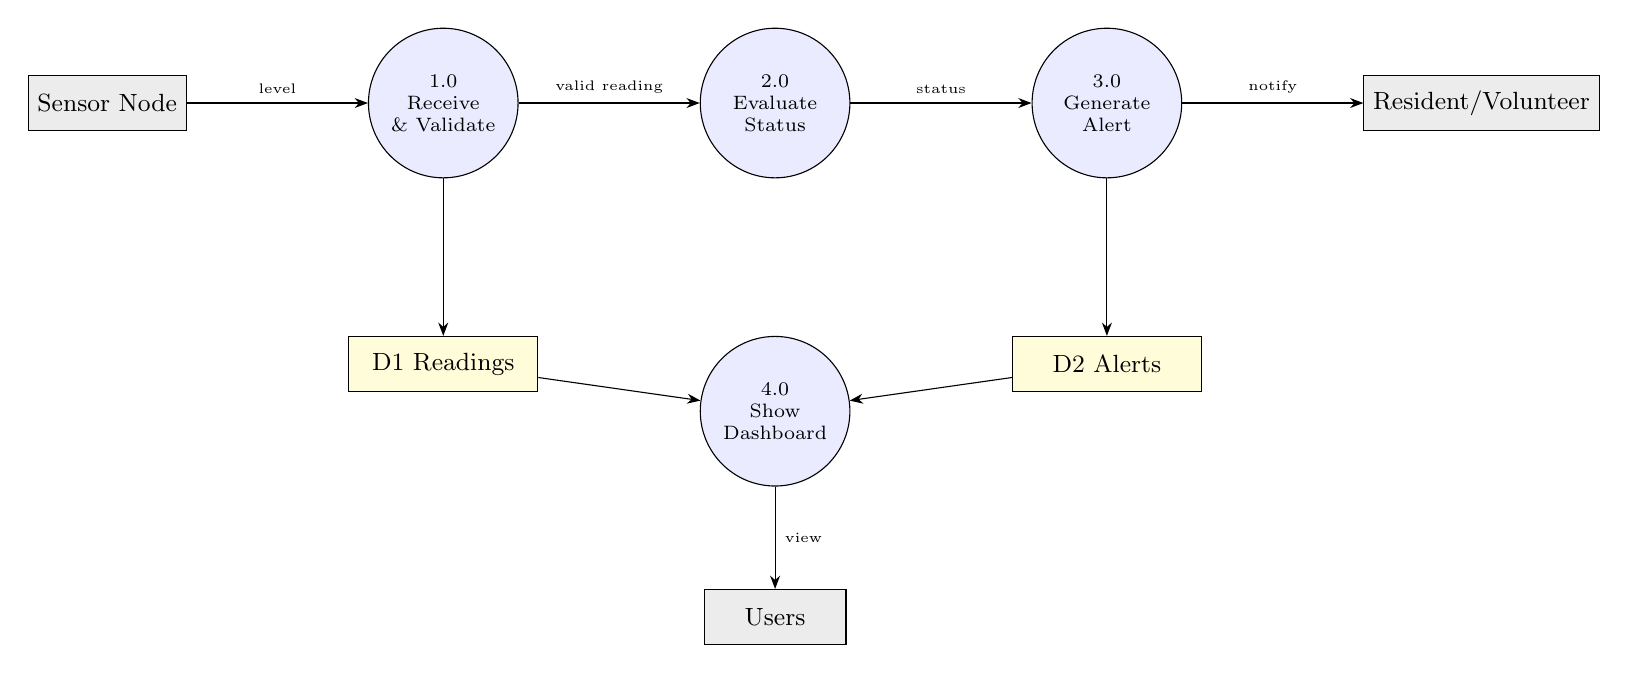
\begin{tikzpicture}[ent/.style={draw,minimum width=1.8cm,minimum height=0.7cm,fill=gray!15,font=\small},proc/.style={draw,circle,align=center,minimum size=1.9cm,fill=blue!8,font=\scriptsize},store/.style={draw,minimum width=2.4cm,minimum height=0.7cm,font=\small,fill=yellow!15},>=Stealth]
\node[ent](sn){Sensor Node};
\node[proc,right=2.3cm of sn](p1){1.0\\Receive\\\& Validate};
\node[proc,right=2.3cm of p1](p2){2.0\\Evaluate\\Status};
\node[proc,right=2.3cm of p2](p3){3.0\\Generate\\Alert};
\node[proc,below=2cm of p2](p4){4.0\\Show\\Dashboard};
\node[store,below=2cm of p1](d1){D1 Readings};
\node[store,below=2cm of p3](d2){D2 Alerts};
\node[ent,right=2.3cm of p3](re){Resident/Volunteer};
\node[ent,below=1.3cm of p4](us){Users};
\draw[->](sn)--node[above,font=\tiny]{level}(p1);
\draw[->](p1)--node[above,font=\tiny]{valid reading}(p2);
\draw[->](p2)--node[above,font=\tiny]{status}(p3);
\draw[->](p1)--(d1);\draw[->](p3)--(d2);
\draw[->](p3)--node[above,font=\tiny]{notify}(re);
\draw[->](d1)--(p4);\draw[->](d2)--(p4);\draw[->](p4)--node[right,font=\tiny]{view}(us);
\end{tikzpicture}}
\caption{DFD Level 1}
\end{figure}

\subsection{Use Case Diagram}
\begin{figure}[H]\centering
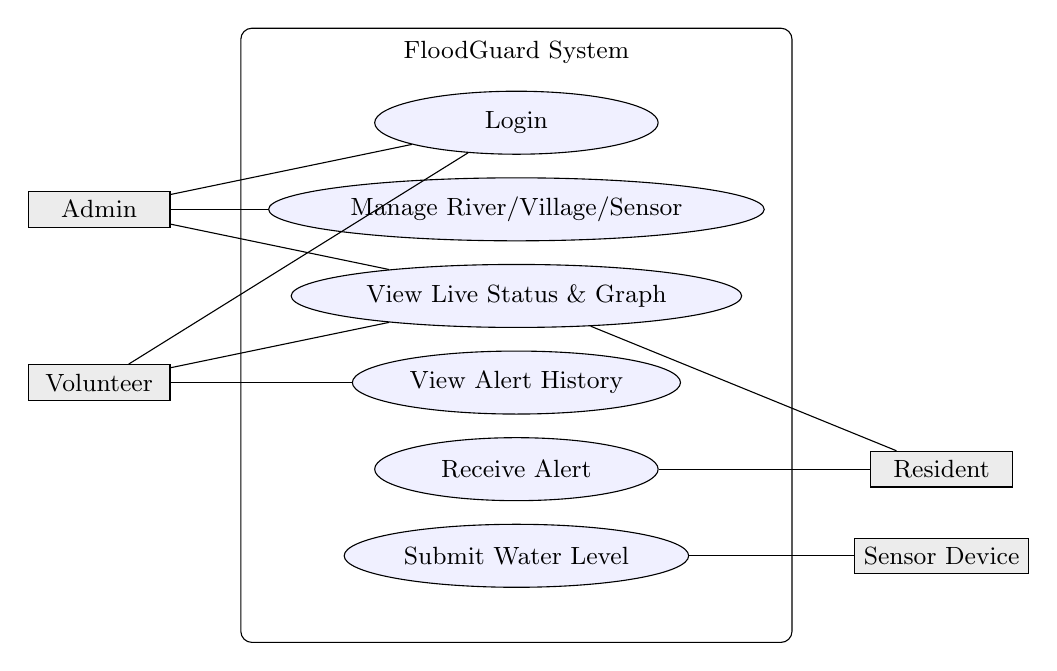
\begin{tikzpicture}[uc/.style={draw,ellipse,minimum width=3.6cm,minimum height=0.8cm,font=\small,fill=blue!6},act/.style={draw,rectangle,fill=gray!15,minimum width=1.8cm,font=\small},>=Stealth]
\draw[rounded corners](2.6,-6.6) rectangle (9.6,1.2);\node at (6.1,0.9){\small FloodGuard System};
\node[uc](u1)at(6.1,0){Login};
\node[uc](u2)at(6.1,-1.1){Manage River/Village/Sensor};
\node[uc](u3)at(6.1,-2.2){View Live Status \& Graph};
\node[uc](u4)at(6.1,-3.3){View Alert History};
\node[uc](u5)at(6.1,-4.4){Receive Alert};
\node[uc](u6)at(6.1,-5.5){Submit Water Level};
\node[act](ad)at(0.8,-1.1){Admin};\node[act](vo)at(0.8,-3.3){Volunteer};
\node[act](re)at(11.5,-4.4){Resident};\node[act](sd)at(11.5,-5.5){Sensor Device};
\draw(ad)--(u1);\draw(ad)--(u2);\draw(ad)--(u3);\draw(vo)--(u1);\draw(vo)--(u3);\draw(vo)--(u4);
\draw(re)--(u5);\draw(re)--(u3);\draw(sd)--(u6);
\end{tikzpicture}
\caption{Use case diagram}
\end{figure}

\subsection{Activity Diagram}
\begin{figure}[H]\centering
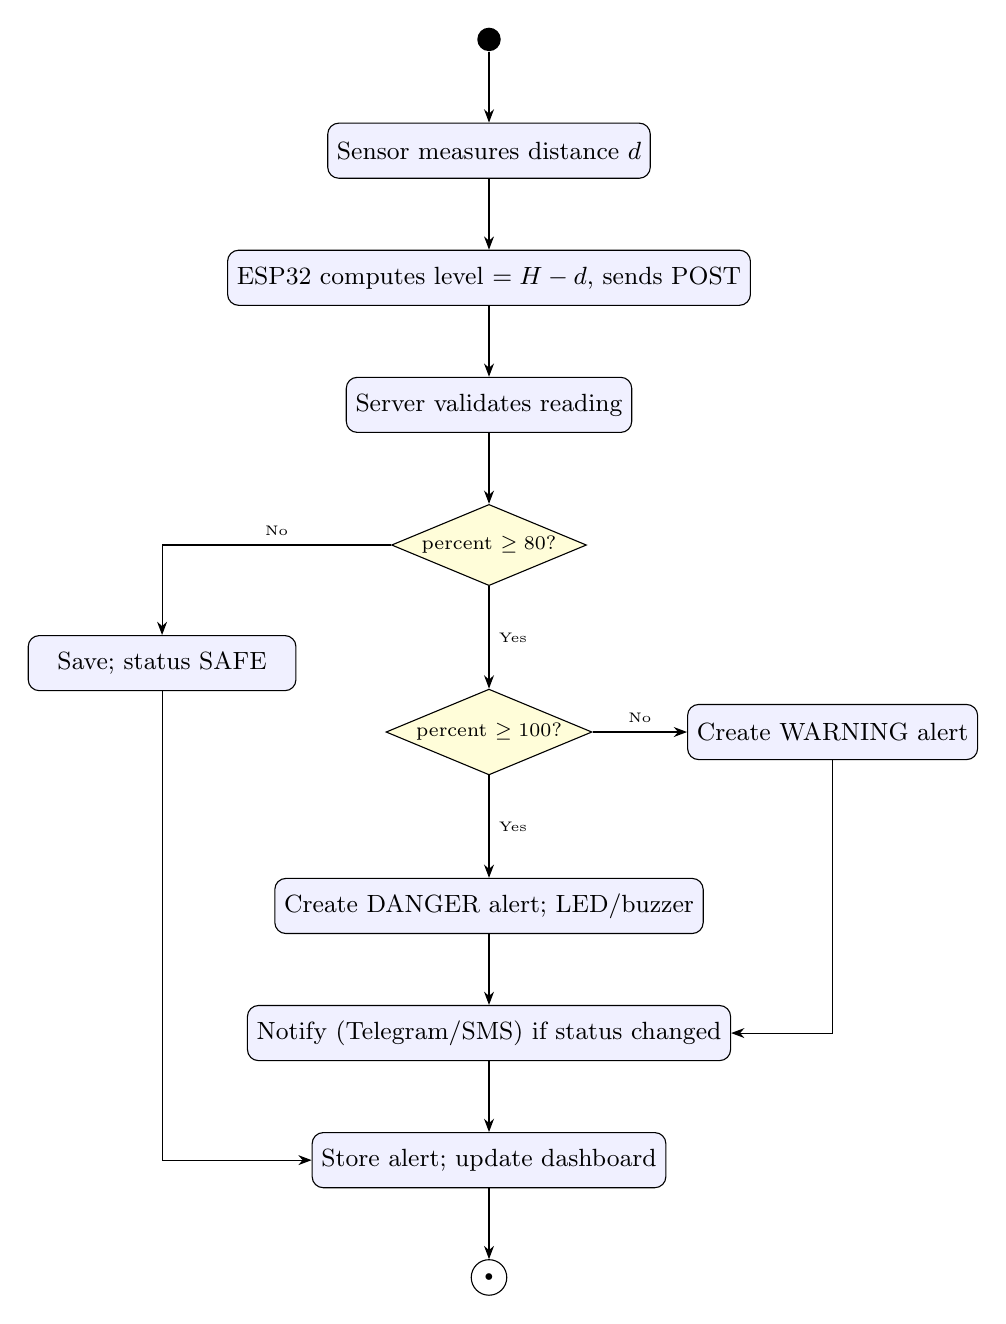
\begin{tikzpicture}[node distance=0.9cm,a/.style={draw,rounded corners,minimum width=3.4cm,minimum height=0.7cm,font=\small,fill=blue!6},d/.style={draw,diamond,aspect=2.4,font=\scriptsize,fill=yellow!15,inner sep=1pt},>=Stealth]
\node[circle,fill=black,inner sep=3pt](st){};
\node[a,below=of st](a1){Sensor measures distance $d$};
\node[a,below=of a1](a2){ESP32 computes level $=H-d$, sends POST};
\node[a,below=of a2](a3){Server validates reading};
\node[d,below=of a3](dc){percent $\ge 80$?};
\node[a,left=1.2cm of dc,yshift=-1.5cm](sf){Save; status SAFE};
\node[d,below=1.3cm of dc](d2){percent $\ge 100$?};
\node[a,right=1.2cm of d2](wr){Create WARNING alert};
\node[a,below=1.3cm of d2](dg){Create DANGER alert; LED/buzzer};
\node[a,below=of dg](nt){Notify (Telegram/SMS) if status changed};
\node[a,below=of nt](sv){Store alert; update dashboard};
\node[circle,draw,inner sep=3pt,below=of sv](en){\tiny$\bullet$};
\draw[->](st)--(a1);\draw[->](a1)--(a2);\draw[->](a2)--(a3);\draw[->](a3)--(dc);
\draw[->](dc)-|node[near start,above,font=\tiny]{No}(sf);
\draw[->](dc)--node[right,font=\tiny]{Yes}(d2);
\draw[->](d2)--node[above,font=\tiny]{No}(wr);\draw[->](d2)--node[right,font=\tiny]{Yes}(dg);
\draw[->](wr)|-(nt);\draw[->](dg)--(nt);\draw[->](nt)--(sv);\draw[->](sv)--(en);
\draw[->](sf)|-($(sv.west)+(-0.3,0)$)--(sv);
\end{tikzpicture}
\caption{Activity diagram: processing a reading}
\end{figure}

\subsection{Entity Relationship Diagram}
\begin{figure}[H]\centering
\resizebox{\textwidth}{!}{%
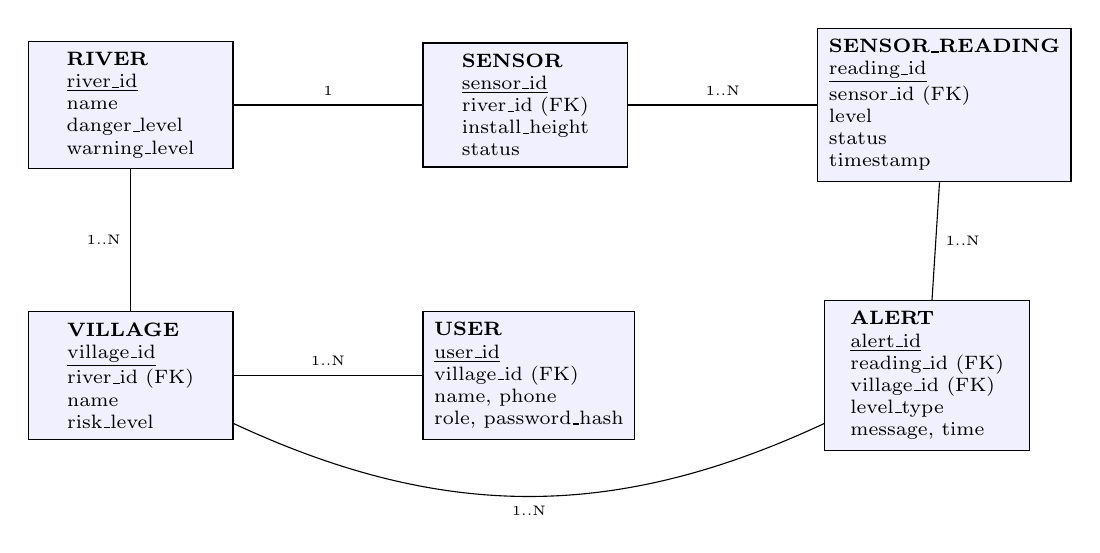
\begin{tikzpicture}[e/.style={draw,rectangle,align=left,font=\scriptsize,fill=blue!6,minimum width=2.6cm,inner sep=4pt},r/.style={draw,diamond,aspect=2,font=\tiny,fill=yellow!15,inner sep=1pt},>=Stealth]
\node[e](ri){\textbf{RIVER}\\\underline{river\_id}\\name\\danger\_level\\warning\_level};
\node[e,right=2.4cm of ri](se){\textbf{SENSOR}\\\underline{sensor\_id}\\river\_id (FK)\\install\_height\\status};
\node[e,right=2.4cm of se](rd){\textbf{SENSOR\_READING}\\\underline{reading\_id}\\sensor\_id (FK)\\level\\status\\timestamp};
\node[e,below=1.8cm of ri](vi){\textbf{VILLAGE}\\\underline{village\_id}\\river\_id (FK)\\name\\risk\_level};
\node[e,right=2.4cm of vi](us){\textbf{USER}\\\underline{user\_id}\\village\_id (FK)\\name, phone\\role, password\_hash};
\node[e,right=2.4cm of us](al){\textbf{ALERT}\\\underline{alert\_id}\\reading\_id (FK)\\village\_id (FK)\\level\_type\\message, time};
\draw(ri)--node[above,font=\tiny]{1}(se);\draw(se)--node[above,font=\tiny]{1..N}(rd);
\draw(ri)--node[left,font=\tiny]{1..N}(vi);\draw(vi)--node[above,font=\tiny]{1..N}(us);
\draw(rd)--node[right,font=\tiny]{1..N}(al);\draw(vi)to[bend right=25]node[below,font=\tiny]{1..N}(al);
\end{tikzpicture}}
\caption{ER diagram (crow's-foot cardinalities shown as 1 and 1..N)}
\end{figure}

\subsection{Class Diagram}
\begin{figure}[H]\centering
\resizebox{\textwidth}{!}{%
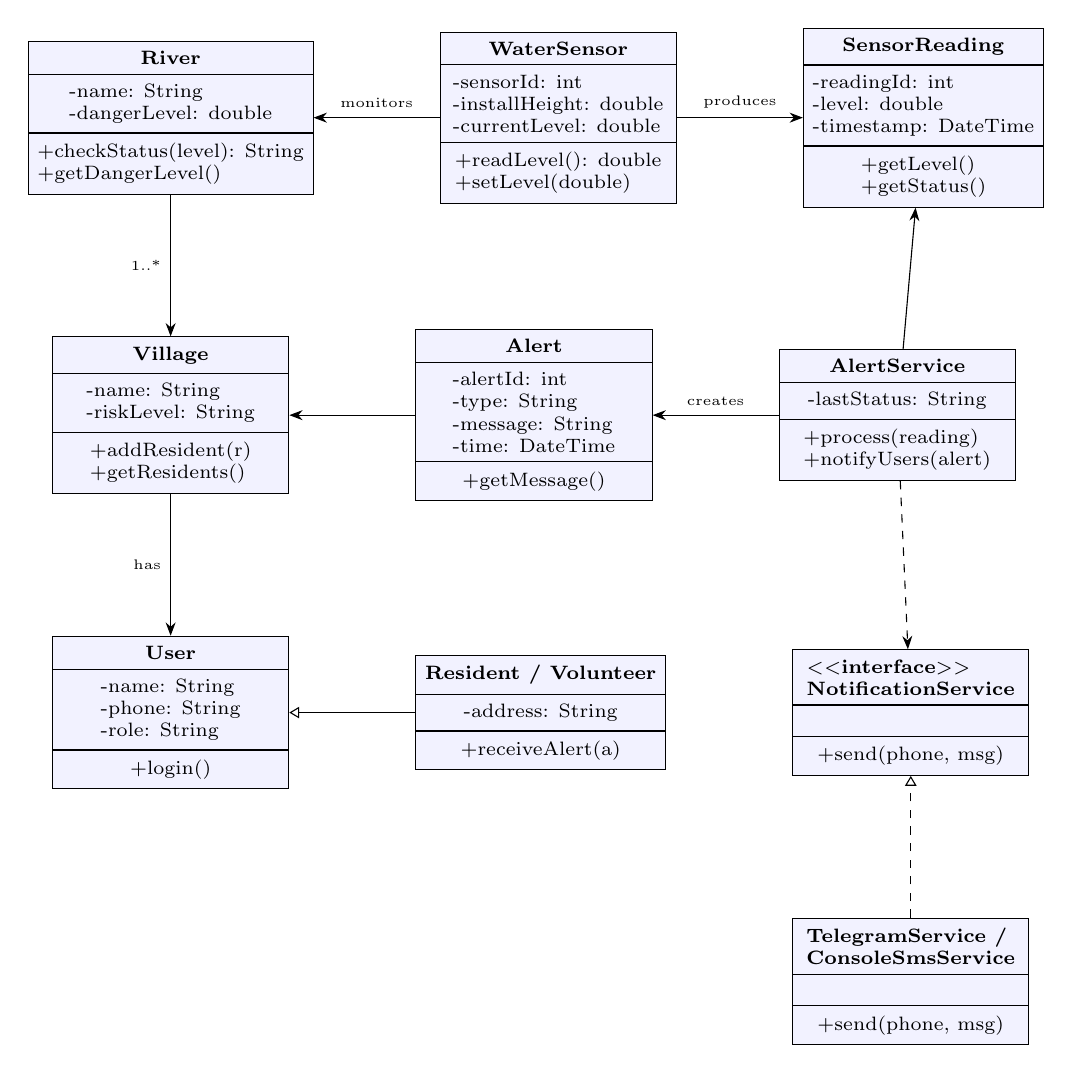
\begin{tikzpicture}[c/.style={draw,rectangle split,rectangle split parts=3,font=\scriptsize,align=left,fill=blue!5,minimum width=3cm},>=Stealth]
\node[c](river){\textbf{River}\nodepart{second}-name: String\\-dangerLevel: double\nodepart{third}+checkStatus(level): String\\+getDangerLevel()};
\node[c,right=1.6cm of river](sensor){\textbf{WaterSensor}\nodepart{second}-sensorId: int\\-installHeight: double\\-currentLevel: double\nodepart{third}+readLevel(): double\\+setLevel(double)};
\node[c,right=1.6cm of sensor](reading){\textbf{SensorReading}\nodepart{second}-readingId: int\\-level: double\\-timestamp: DateTime\nodepart{third}+getLevel()\\+getStatus()};
\node[c,below=1.8cm of river](village){\textbf{Village}\nodepart{second}-name: String\\-riskLevel: String\nodepart{third}+addResident(r)\\+getResidents()};
\node[c,right=1.6cm of village](alert){\textbf{Alert}\nodepart{second}-alertId: int\\-type: String\\-message: String\\-time: DateTime\nodepart{third}+getMessage()};
\node[c,right=1.6cm of alert](svc){\textbf{AlertService}\nodepart{second}-lastStatus: String\nodepart{third}+process(reading)\\+notifyUsers(alert)};
\node[c,below=1.8cm of village](user){\textbf{User}\nodepart{second}-name: String\\-phone: String\\-role: String\nodepart{third}+login()};
\node[c,right=1.6cm of user](res){\textbf{Resident / Volunteer}\nodepart{second}-address: String\nodepart{third}+receiveAlert(a)};
\node[c,right=1.6cm of res](ns){\textbf{$<<$interface$>>$}\\\textbf{NotificationService}\nodepart{second}\nodepart{third}+send(phone, msg)};
\node[c,below=1.8cm of ns](tg){\textbf{TelegramService /}\\\textbf{ConsoleSmsService}\nodepart{second}\nodepart{third}+send(phone, msg)};
\draw[->](sensor)--node[above,font=\tiny]{monitors}(river);
\draw[->](sensor)--node[above,font=\tiny]{produces}(reading);
\draw[->](river)--node[left,font=\tiny]{1..*}(village);
\draw[->](svc)--node[above,font=\tiny]{creates}(alert);
\draw[->](svc)--(reading);
\draw[->](alert)--(village);
\draw[->,dashed](svc)--(ns);
\draw[-{Triangle[open]}](res)--(user);
\draw[-{Triangle[open]},dashed](tg)--(ns);
\draw[->](village)--node[left,font=\tiny]{has}(user);
\end{tikzpicture}}
\caption{Class diagram}
\end{figure}

\subsection{Object Diagram}
\begin{figure}[H]\centering
\resizebox{\textwidth}{!}{%
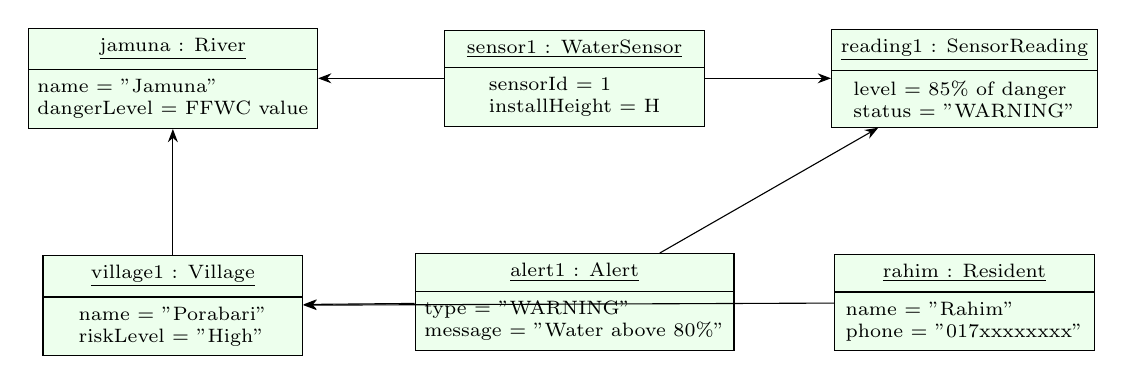
\begin{tikzpicture}[o/.style={draw,rectangle split,rectangle split parts=2,font=\scriptsize,align=left,fill=green!7,minimum width=3.3cm},>=Stealth]
\node[o](jr){\underline{jamuna : River}\nodepart{second}name = "Jamuna"\\dangerLevel = FFWC value};
\node[o,right=1.6cm of jr](s1){\underline{sensor1 : WaterSensor}\nodepart{second}sensorId = 1\\installHeight = H};
\node[o,right=1.6cm of s1](r1){\underline{reading1 : SensorReading}\nodepart{second}level = 85\% of danger\\status = "WARNING"};
\node[o,below=1.6cm of jr](v1){\underline{village1 : Village}\nodepart{second}name = "Porabari"\\riskLevel = "High"};
\node[o,below=1.6cm of s1](a1){\underline{alert1 : Alert}\nodepart{second}type = "WARNING"\\message = "Water above 80\%"};
\node[o,below=1.6cm of r1](u1){\underline{rahim : Resident}\nodepart{second}name = "Rahim"\\phone = "017xxxxxxxx"};
\draw[->](s1)--(jr);\draw[->](s1)--(r1);\draw[->](a1)--(r1);\draw[->](a1)--(v1);\draw[->](u1)--(v1);\draw[->](v1)--(jr);
\end{tikzpicture}}
\caption{Object diagram (sample snapshot)}
\end{figure}

%================ 11 IMPLEMENTATION ================
\section{Simple Interface Implementation Plan}
The interface is a browser dashboard served by a Java Servlet. At least five classes from the class diagram are implemented: \texttt{River}, \texttt{WaterSensor}, \texttt{SensorReading}, \texttt{Alert}, \texttt{AlertService} (plus \texttt{NotificationService} implementations).
\begin{lstlisting}[language=Java,caption={Status logic in River (core of the system)}]
public class River {
    private String name;
    private double dangerLevel;
    public River(String name, double dangerLevel) {
        this.name = name; this.dangerLevel = dangerLevel;
    }
    public String checkStatus(double level) {
        double p = level / dangerLevel * 100;
        if (p >= 100) return "DANGER";
        if (p >= 80)  return "WARNING";
        return "SAFE";
    }
}
\end{lstlisting}
\textbf{Dashboard shows:} river name, current level, status colour (green/yellow/red), progress bar, level-versus-time graph, alert list, and a ``Start Simulation'' button.

\textbf{ESP32 firmware (summary):} read HC-SR04, compute $H-d$, show status on green/yellow/red LEDs and buzzer, and send the level to \texttt{/data} using HTTP POST.

\section{Testing Plan}
\begin{table}[H]\centering\small
\begin{tabular}{@{}lllp{4cm}@{}}\toprule \textbf{ID} & \textbf{Input} & \textbf{Expected} & \textbf{Type}\\\midrule
T1 & 50\% of danger level & SAFE, green & Unit (JUnit)\\
T2 & 85\% of danger level & WARNING, yellow, alert & Unit\\
T3 & 105\% of danger level & DANGER, red, alert, buzzer & Unit/System\\
T4 & Same status repeated & No duplicate notification & Unit\\
T5 & Telegram unreachable & Server continues, console fallback & System\\
T6 & Invalid/negative reading & Rejected & Unit\\\bottomrule
\end{tabular}\caption{Sample test cases}\end{table}

%================ 12 CONCLUSION ================
\section{Conclusion and Future Work}
FloodGuard demonstrates a practical, low-cost IoT approach to village-level flood early warning, developed with a structured software engineering process (Incremental model), complete UML modelling and a realistic schedule. The prototype shows the full chain from sensing to alerting while being transparent about what is emulated. Future work includes LoRa/GSM connectivity, solar power, multiple nodes, a mobile app, integration of rainfall and upstream data, and machine learning based forecasting.

\end{document}
